\documentclass[tikz,border=3pt]{standalone}
\usepackage[utf8]{inputenc}
\usepackage[T1]{fontenc}
\usepackage{lmodern}
\renewcommand{\familydefault}{\sfdefault}
\usepackage{sansmath}\sansmath
\usepackage{chemfig}
\usepackage{pgfplots}\pgfplotsset{compat=1.18,/pgf/number format/use comma,/pgf/number format/1000 sep={.}}
\usetikzlibrary{arrows.meta,calc,positioning,decorations.pathmorphing,patterns}
% paleta del sitio
\definecolor{nar}{HTML}{E8680C}\definecolor{narc}{HTML}{FFB35C}\definecolor{hielo}{HTML}{FFF3E8}
\definecolor{tinta}{HTML}{1D1D1F}\definecolor{gris}{HTML}{6E6E73}\definecolor{lila}{HTML}{7C5CF0}
\definecolor{azul}{HTML}{2F6FD6}\definecolor{menta}{HTML}{17A673}\definecolor{coral}{HTML}{E8342A}
\begin{document}
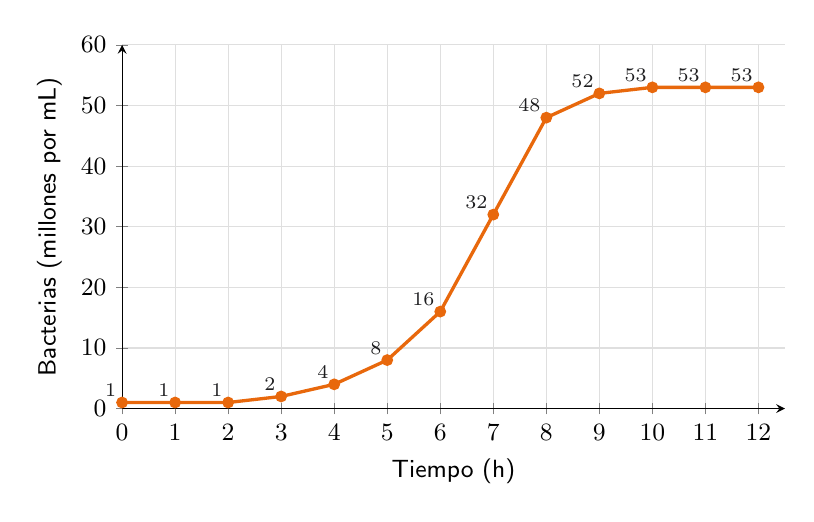
\begin{tikzpicture}[font=\small]
\begin{axis}[width=10cm,height=6.2cm,axis lines=left,xmin=0,xmax=12.5,ymin=0,ymax=60,xtick={0,1,...,12},ytick={0,10,...,60},
  grid=major,grid style={gray!25},xlabel={Tiempo (h)},ylabel={Bacterias (millones por mL)},clip=false,
  nodes near coords,every node near coord/.append style={font=\scriptsize,text=tinta,anchor=south east,inner sep=1.5pt}]
\addplot[nar,very thick,mark=*,mark options={fill=nar,scale=0.75}] coordinates {(0,1)(1,1)(2,1)(3,2)(4,4)(5,8)(6,16)(7,32)(8,48)(9,52)(10,53)(11,53)(12,53)};
\end{axis}
\end{tikzpicture}
\end{document}
